\section{GraphWalker Framework}

\begin{figure*}[t]
  \centering
  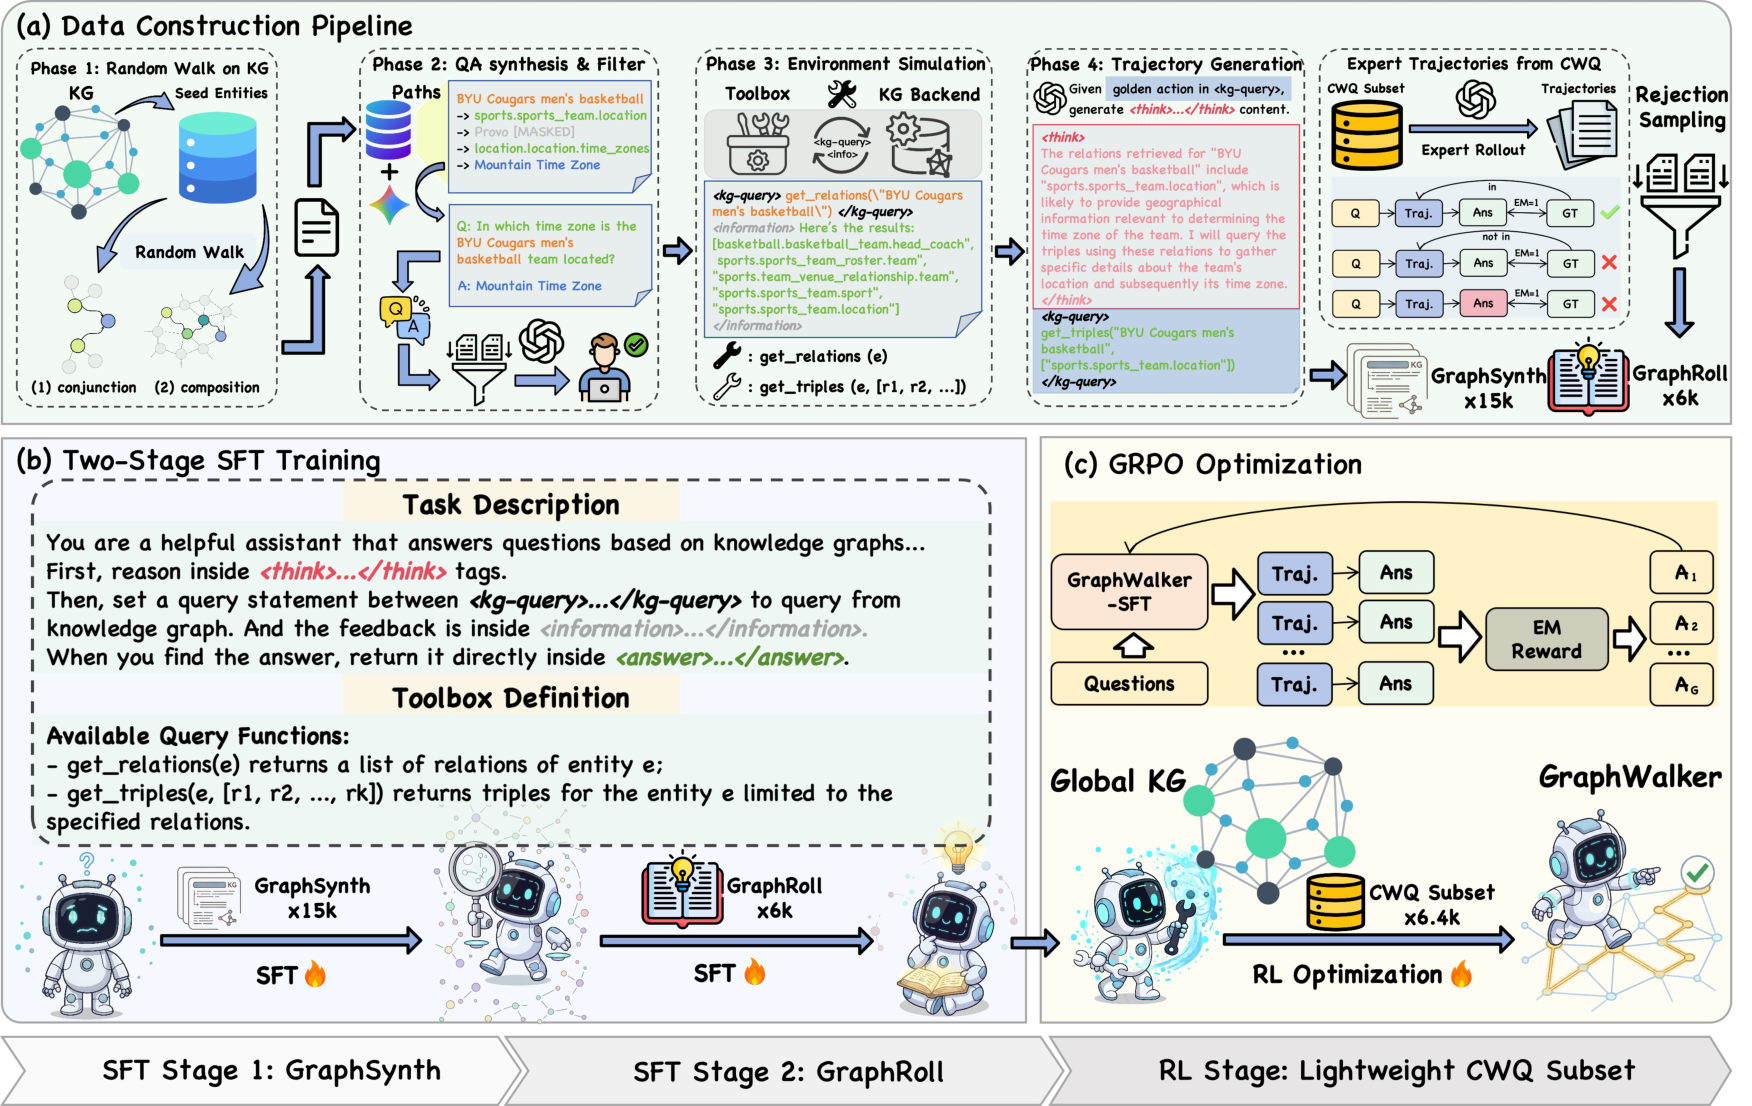
\includegraphics[width=\textwidth]{figures/graphwalker_overview.pdf}
  \vspace{-16pt}
  \caption{
  \textbf{Overview of our proposed GraphWalker.} 
  \textbf{(a) Data Construction:} a multi-phase pipeline for GraphSynth-15k and outcome-based rejection sampling for GraphRoll-6k. 
  \textbf{(b) Two-Stage SFT:} Stage 1 establishes a broad exploration prior, while Stage 2 instills reflection and error recovery. 
  \textbf{(c) RL Optimization:} GRPO with a simple exact-match reward unlocks a higher performance ceiling enabled by the two-stage SFT prior.}
  \label{fig:overview}
  \vspace{-14pt}
\end{figure*}


In this section, we present the GraphWalker framework, which consists of three components: the agentic environment, the data construction pipeline, and the training procedure. Figure~\ref{fig:overview} provides an overview of the full data construction and training pipeline.

\subsection{Agentic Initialization}
\label{sec:env_init}

\textbf{Environment.}
Following prior agentic KGQA systems \citep{sun2023think,jiang2025kg}, 
we formalize the KG as an executable environment backed by a \textit{SPARQL} endpoint. Unlike approaches that operate on pre-defined subgraphs, the agent interacts directly with the global KG in real time during both training and inference. 
This design exposes the agent to the full structural complexity of real-world KGs, including large branching factors and long-tail relations, which encourages more robust reasoning strategies.

\textbf{Toolbox.}
To interact with this environment, we equip the agent with two primitive tools:
(1)~$\textbf{get\_relations}(e)$ returns all relations incident 
to entity $e$, allowing the agent to survey the local neighborhood 
before selecting a retrieval direction.
(2)~$\textbf{get\_triples}(e, \mathcal{R}')$ returns all triples 
whose head or tail is $e$ and whose relation belongs to a subset 
$\mathcal{R}' \subseteq \mathcal{R}_{\{e\}}$ selected from the 
preceding \textbf{get\_relations} observation, enabling targeted 
and efficient KG traversal.

\textbf{Agent Loop.}
At each turn $t \leq T$, where $T$ is the maximum number of 
interaction turns, the agent is conditioned on the current state 
$s_t = (q, \tau_{t-1})$, where $q$ is the input question and 
$\tau_{t-1} = \{(c_i, a_i, o_i)\}_{i=1}^{t-1}$ is the interaction 
history up to the preceding turn. Here, $c_i$ denotes the model's 
internal reasoning process at turn $i$, $a_i$ the executed action, 
and $o_i$ the resulting observation.
Given $s_t$, the agent produces a response consisting of two parts: 
(1)~an internal reasoning process $c_t$, enclosed in 
\texttt{<think>}\ldots\texttt{</think>}, which reflects on the current 
state and determines the next action; and (2)~an action $a_t$, which 
is either a KG retrieval query enclosed in 
\texttt{<kg-query>}\ldots\texttt{</kg-query>}, or a final answer 
enclosed in \texttt{<answer>}\ldots\texttt{</answer>} when sufficient 
evidence has been gathered.
The executor processes $a_t$ on the KG $\mathcal{G}$ and returns the 
retrieval result as an observation $o_t$, enclosed in 
\texttt{<information>}\ldots\texttt{</information>} and appended to 
the trajectory. The full turn record $(c_t, a_t, o_t)$ is then 
appended to $\tau_t$.




\subsection{Data Construction}
\label{sec:data_construction}

In this section, we describe the construction of two complementary training corpora, \textbf{GraphSynth-15k} and \textbf{GraphRoll-6k}.
GraphSynth-15k focuses on broad structural coverage for exploration, while GraphRoll-6k emphasizes reflection and error recovery.


\subsubsection{GraphSynth: Diverse Trajectory Synthesis}

We first construct GraphSynth, a 15k corpus of KG-grounded interaction trajectories, using a four-phase pipeline designed to promote structural diversity, incorporate weak supervision, and simulate realistic interaction.

\textbf{Phase 1: Constrained Random Walk on KG.}

We first extract the predicate set $\mathcal{P}$ and the seed entity set $\mathcal{E}$ from the SPARQL logical forms of all the training splits of CWQ, WebQSP, and GrailQA. 
Despite using seen atomic relations, our CRW systematically recombines them into unobserved topological structures to drive compositional generalization.
Starting from a seed entity $e_0 \in \mathcal{E}$, we perform constrained random walks over relations in $\mathcal{P}$ to generate structurally diverse reasoning paths.
As shown in Figure~\ref{fig:crw_paths}(a), we introduce two complementary families of reasoning structures. \textbf{Composition chains} span \textbf{2--5 hops}, capturing sequential multi-hop exploration patterns. \textbf{Conjunction graphs} (denoted as \textbf{2I} in Figure~\ref{fig:crw_paths}(a)) originate from two distinct topic entities and converge on a shared target entity. 
Formally, each transition samples a relation--node pair subject to the predicate constraint:
\begin{equation}
r_t \in \mathcal{P}, \qquad e_{t+1}\in\mathcal{N}(e_t,r_t), \qquad d_{\min} \leq |\mathcal{N}(e_t,r_t)| \leq d_{\max},
\label{eq:crw_transition}
\end{equation}
where $\mathcal{N}(e_t,r_t)$ denotes the set of neighbors reachable from $e_t$ via relation $r_t$, and the cardinality constraint $d_{\min} \leq |\mathcal{N}(e_t,r_t)| \leq d_{\max}$ ensures that sampled relations are neither trivially unique nor excessively branching, thereby promoting structural diversity while avoiding degenerate or uninformative paths.


\begin{figure}[t]
  \centering
  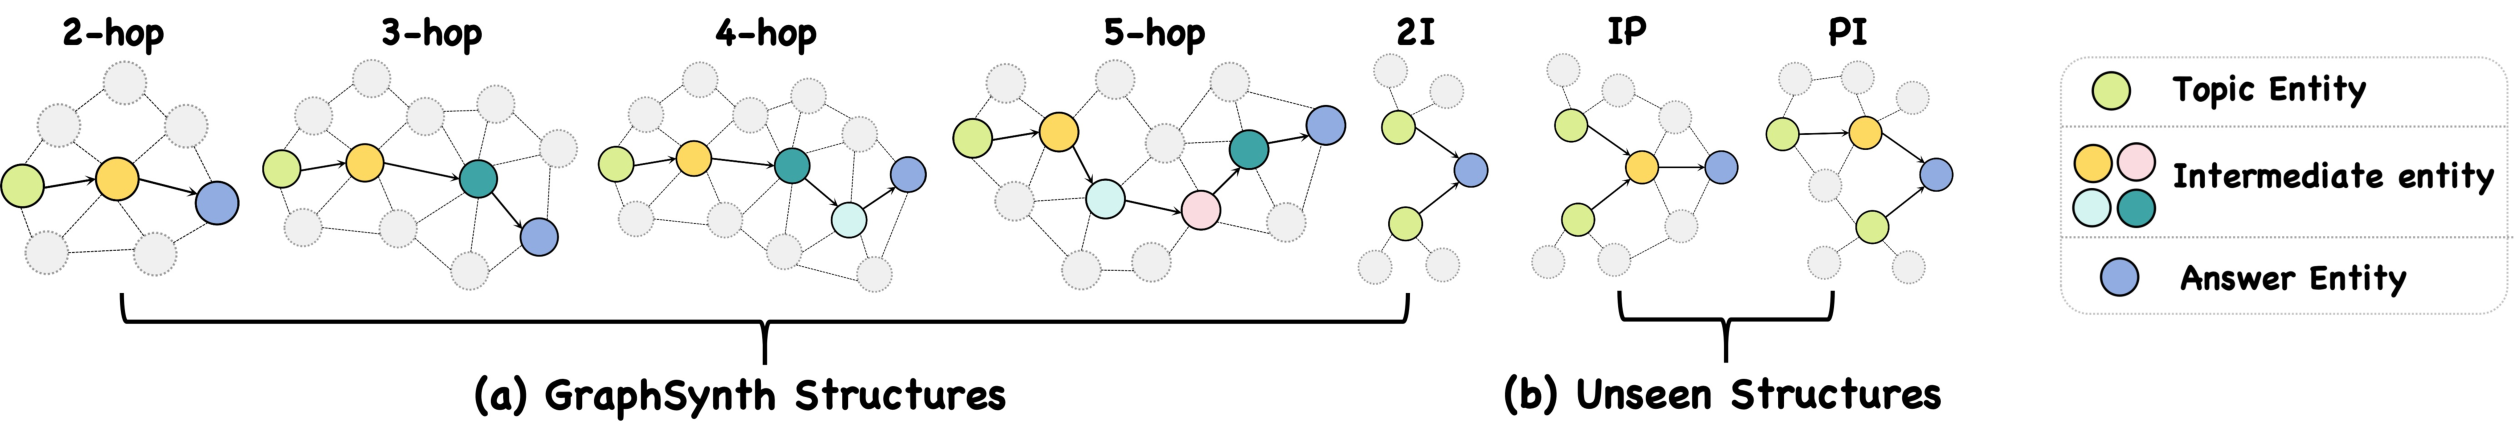
\includegraphics[width=\linewidth]{figures/rw_paths.pdf}
  \caption{Representative interaction paths generated by constrained random walks.}
  \label{fig:crw_paths}
  \vspace{-14pt}
\end{figure}




\textbf{Phase 2: Question Synthesis and Semantic Filtering.}

As shown in Figure~\ref{fig:overview} (Phase 2), for each reasoning path, we use \texttt{Gemini-2.5-Pro} \citep{comanici2025gemini25pushingfrontier} to generate a natural language question. 
To prevent information leakage, we \textbf{mask intermediate entities} (as $entity_1, entity_2, \dots$) along reasoning paths. For example, reasoning path "$\text{BYU Cougars men's basketball} \xrightarrow{\texttt{team.location}} entity_1 \xrightarrow{\texttt{time\_zones}} \text{Mountain Time Zone}$" yields: "In which time zone is the BYU Cougars men's basketball team located?"
To ensure data quality, we apply \textbf{LLM-based semantic filtering} using \texttt{GPT-4o-mini} \citep{hurst2024gpt}, which scores each question along three dimensions: 
(1) \textbf{reasoning path completeness}, 
(2) \textbf{question-path relevance}, 
and (3) \textbf{question semantic coherence}. 
Questions with an average score below $9$ out of $10$ are discarded.
In case of test-set leakage, we also verify that GraphSynth contains negligible semantic overlap with all the benchmarks (details in Appendix~\ref{app:contamination}).

To further validate the model's generalization capabilities, we also construct our own evaluation set, \textit{GraphWalkerBench},  which contains unseen reasoning structures in the GraphSynth dataset (shown in Figure~\ref{fig:crw_paths}(b), details in Appendix~\ref{app:datasets}).



\textbf{Phase 3: Environment Feedback Simulation.}

To faithfully simulate inference-time interaction, we execute each CRW path as a sequence of SPARQL queries against the full KG. We apply the same retrieval and filtering pipeline used at inference time, including \textbf{BM25}~\citep{bm25} candidate retrieval and \textbf{LLM-based relation reranking} (e.g., \texttt{Qwen2.5-7B-Instruct}). 
At each step $t$, we prompt an LLM to rerank the top-$k$ relations and up to 5 triples per relation as the observation $o_t$.

\textbf{Phase 4: Agent Thought Generation.}

As shown in Figure~\ref{fig:overview} (Phase 4), at each step $t$, given the current state $s_t$ and the corresponding oracle next action $a_{t}$, we use \texttt{GPT-4o-mini} as a rationale generator to generate the reasoning process $c_t$, i.e., chain-of-thought rationales that explain the selection of subsequent actions under the current context.
The resulting tuples $(c_t, a_t, o_t)$ are then assembled into complete interaction trajectories $\tau$, forming \textbf{GraphSynth-15k}.


\subsubsection{GraphRoll: Expert Trajectory Collection}
We then construct a smaller set of expert trajectories that demonstrate reflection and error recovery.
Given the complexity and diversity of CWQ, we sample a representative subset of 6k questions via stratified sampling across different question types to ensure balanced training coverage.
For each question, we use \texttt{GPT-4o-mini} as the expert model 
to generate high-quality trajectories that involve reflecting on 
uninformative observations and backtracking from dead ends.
We apply \textbf{outcome-based rejection sampling} based on two 
complementary criteria ensuring factual correctness and KG grounding:
\textbf{(1) Answer Correctness:} the predicted answer must be correct ($EM=1$).
\textbf{(2) Evidence Grounding:} all predicted answers must appear in the 
observation history $\{o_0, \ldots, o_T\}$, ensuring every answer is 
grounded in the retrieved KG evidence rather than parametric knowledge.
The resulting trajectories form \textbf{GraphRoll-6k}.



\subsection{GraphWalker Training}
\label{sec:training}

We adopt a two-stage SFT cold start followed by RL training. 
The first stage equips the agent with general exploration skills, 
the second cultivates reflection and error recovery, and RL 
subsequently aligns long-horizon decision making.
We parameterize the agent policy as an autoregressive language 
model $\pi_\theta$.
Specifically, in stage 1 and stage 2, the model is optimized using a next-token prediction objective over agentic interaction sequences, while treating \texttt{<information>} blocks as environmental context rather than learning targets:
\begin{equation}
\mathcal{L}(\theta) = 
-\sum_{t \in \mathcal{I}_{\text{agent}}} 
\log P_\theta(x_t \mid x_{<t}),
\end{equation}
where $\mathcal{I}_{\text{agent}}$ indexes tokens in the 
\texttt{<think>}, \texttt{<kg-query>}, and \texttt{<answer>} blocks.

\textbf{SFT Stage 1: Learning to Reason and Explore on Diverse KGs.}

In stage 1, we first train the agent on \textbf{GraphSynth-15k}. This stage aims to internalize robust navigation behaviors and 
reliable tool-invocation patterns under realistic retrieval noise, 
while treating KG retrieval results as environmental observations.


\newpage
\textbf{SFT Stage 2: Learning to Reflect and Recover from Errors.}

In stage 2, we fine-tune the model on \textbf{GraphRoll-6k}. 
Unlike stage 1, which emphasizes broad exploration, the expert trajectories in GraphRoll-6k contain explicit instances of error detection and reasoning recovery, guiding the model to develop more deliberate and self-corrective interaction strategies.


\textbf{RL Stage: Unlocking the Performance Ceiling}

Building on the two-stage SFT cold-start model, we apply 
RL to push the agent's performance beyond the SFT ceiling 
through autonomous exploration.
We train the model on a uniformly sampled CWQ subset using Group Relative Policy Optimization (GRPO) \citep{Guo_2025} with a sparse, trajectory-level exact match reward:
\begin{equation}
R(\tau) = s_{\text{EM}}(\tau) \in \{0, 1\}.
\end{equation}
Since our two-stage SFT already establishes an exploration and reflection prior, this sparse reward is sufficient to drive further policy improvement without dense intermediate supervision. The GRPO objective function is:

{\small
\begin{equation}
\mathcal{J}_{\text{GRPO}}(\theta) = \mathbb{E}_{q,\{\tau^{(i)}\}} \left[
  \frac{1}{N} \sum_{i=1}^{N} \frac{1}{|\tau^{(i)}|}
  \sum_{j=1}^{|\tau^{(i)}|}
  \min\!\left( \rho_{i,j} \hat{A}_{i,j},\;
  \mathrm{clip}(\rho_{i,j}, 1-\epsilon , 1+\epsilon)\, \hat{A}_{i,j} \right)
\right] - \beta\,\mathbb{D}_{\mathrm{KL}}(\pi_\theta \| \pi_{\text{ref}}),
\label{eq:grpo}
\end{equation}
}

where $\rho_{i,j}=\frac{\pi_\theta(a_{i,j}|s_{i,j})}{\pi_{\text{old}}(a_{i,j}|s_{i,j})}$ 
is the importance ratio, $\hat{A}_{i,j}$ is the group-normalized 
advantage, and $\pi_{\text{ref}}$ is the two-stage SFT model used as the KL reference policy.


